% Source for docs/static/img/ac-training.svg. Rebuild from the repository root:
%   pdflatex -output-directory=/tmp docs/scripts/ac-training.tex
%   pdf2svg /tmp/ac-training.pdf docs/static/img/ac-training.svg
%   python3 docs/scripts/prepare_rollout_svgs.py
\documentclass[tikz,border=3pt]{standalone}
\usepackage{amsmath,amssymb,bm}
\usetikzlibrary{arrows.meta,positioning,calc,fit}

\colorlet{agentA}{red!80!black}     % agent 1: policy, prompts, responses, loss
\colorlet{agentB}{blue!80!black}    % agent 2
\colorlet{learned}{orange!80!black} % learned evaluators: critic, reward model
\colorlet{update}{green!50!black}   % gradients and parameter updates

\tikzset{
  >={Stealth[length=3.2pt,width=3pt]},
  box/.style={draw, line width=1pt, inner sep=2.5pt, minimum height=13pt},
  policy/.style={box, rounded corners=3pt, minimum width=30pt},
  flow/.style={->, line width=.8pt},
  note/.style={font=\scriptsize, align=left},
  label/.style={anchor=west, font=\footnotesize},
}

% One turn of MAAC (top) and IAC (bottom), left to right: the agents' responses
% share one reward, and the critics turn it into TD errors that weight each agent's
% own policy gradient. Columns are animation stages.
\begin{document}
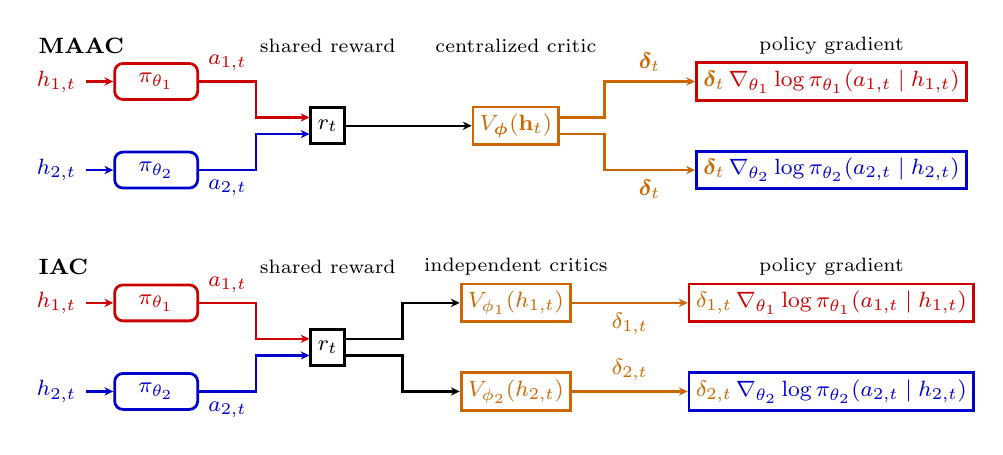
\begin{tikzpicture}[x=1pt, y=1pt, font=\footnotesize]
  % Agents, shared reward, and edges common to both panels; #1 is the panel center.
  \newcommand{\rollout}[1]{%
    \node[agentA] (h1) at (0,#1+16) {$h_{1,t}$};
    \node[agentB] (h2) at (0,#1-16) {$h_{2,t}$};
    \node[policy, agentA] (p1) at (36,#1+16) {$\pi_{\theta_1}$};
    \node[policy, agentB] (p2) at (36,#1-16) {$\pi_{\theta_2}$};
    \draw[flow, agentA] (h1) -- (p1);
    \draw[flow, agentB] (h2) -- (p2);
    \node[box] (r) at (98,#1) {$r_t$};
    \node[note] at (98,#1+29) {shared reward};
    \draw[flow, agentA] (p1.east) -- node[above] {$a_{1,t}$} (72,#1+16) |- ([yshift=3pt]r.west);
    \draw[flow, agentB] (p2.east) -- node[below] {$a_{2,t}$} (72,#1-16) |- ([yshift=-3pt]r.west);
  }

  % MAAC: one centralized critic gives every agent the same TD error.
  \node[label, font=\footnotesize\bfseries] at (-10,29) {MAAC};
  \rollout{0}
  \node[box, learned] (c) at (166,0) {$V_{\boldsymbol{\phi}}(\mathbf{h}_t)$};
  \node[note] at (166,29) {centralized critic};
  \draw[flow] (r) -- (c);
  \node[box, agentA] (g1) at (280,16)
    {$\textcolor{learned}{\boldsymbol{\delta}_t}\,\nabla_{\theta_1}\log\pi_{\theta_1}(a_{1,t}\mid h_{1,t})$};
  \node[box, agentB] (g2) at (280,-16)
    {$\textcolor{learned}{\boldsymbol{\delta}_t}\,\nabla_{\theta_2}\log\pi_{\theta_2}(a_{2,t}\mid h_{2,t})$};
  \node[note] at (280,29) {policy gradient};
  \draw[flow, learned] ([yshift=3pt]c.east) -- (198,3) |- node[pos=.75, above] {$\boldsymbol{\delta}_t$} (g1.west);
  \draw[flow, learned] ([yshift=-3pt]c.east) -- (198,-3) |- node[pos=.75, below] {$\boldsymbol{\delta}_t$} (g2.west);

  % IAC: each agent's critic sees only that agent's history and gives its own TD error.
  \node[label, font=\footnotesize\bfseries] at (-10,-51) {IAC};
  \rollout{-80}
  \node[box, learned] (c1) at (166,-64) {$V_{\phi_1}(h_{1,t})$};
  \node[box, learned] (c2) at (166,-96) {$V_{\phi_2}(h_{2,t})$};
  \node[note] at (166,-51) {independent critics};
  \node[note] at (280,-51) {policy gradient};
  \draw[flow] ([yshift=3pt]r.east) -- (125,-77) |- (c1.west);
  \draw[flow] ([yshift=-3pt]r.east) -- (125,-83) |- (c2.west);
  \node[box, agentA] (g1) at (280,-64)
    {$\textcolor{learned}{\delta_{1,t}}\,\nabla_{\theta_1}\log\pi_{\theta_1}(a_{1,t}\mid h_{1,t})$};
  \node[box, agentB] (g2) at (280,-96)
    {$\textcolor{learned}{\delta_{2,t}}\,\nabla_{\theta_2}\log\pi_{\theta_2}(a_{2,t}\mid h_{2,t})$};
  \draw[flow, learned] (c1) -- node[below] {$\delta_{1,t}$} (g1);
  \draw[flow, learned] (c2) -- node[above] {$\delta_{2,t}$} (g2);
\end{tikzpicture}
\end{document}
